\documentclass[pdf]{beamer}
\mode<presentation>{}
\usepackage{colortbl}
\usepackage{tikz}
\usetikzlibrary{positioning}
\usetikzlibrary{arrows}
\usepackage[utf8]{inputenc}
\usepackage[T1]{fontenc}
\usepackage{mathtools}
\DeclarePairedDelimiter\ceil{\lceil}{\rceil}
\DeclarePairedDelimiter\floor{\lfloor}{\rfloor}

\definecolor{mygreen}{rgb}{0,0.6,0}
\definecolor{mygray}{rgb}{0.5,0.5,0.5}
\definecolor{mymauve}{rgb}{0.58,0,0.82}

\setbeamertemplate{footline}[frame number]

\usepackage{listingsutf8}
\lstset{ %
	backgroundcolor=\color{white},
	basicstyle=\footnotesize,
	breakatwhitespace=false,
	breaklines=true,
	captionpos=b,
	commentstyle=\color{mygreen},
	deletekeywords={},
	escapeinside={\%*}{*)},
	extendedchars=true,
	frame=none,
	keepspaces=true,
	keywordstyle=\color{blue},
	language=Java,
	morekeywords={},
	numbers=none,
	numbersep=0pt,
	numberstyle=\tiny\color{mygray},
	rulecolor=\color{black},
	showspaces=false,
	showstringspaces=false,
	showtabs=false,
	stepnumber=0,
	stringstyle=\color{mymauve},
	tabsize=2,
	belowskip=0pt,
	aboveskip=0pt,
}

%% preamble
\title{Computationnal geometry}
\author{Guillaume \textsc{Derval}}

\begin{document}

%% title frame
\begin{frame}
\titlepage
\end{frame}

{
\begin{frame}{Table of Contents}
\tableofcontents[]
\end{frame}
}

\AtBeginSection[]
{
\begin{frame}{Table of Contents}
\tableofcontents[currentsection]
\end{frame}
}

\AtBeginSubsection[]
{
\begin{frame}{Table of Contents}
\tableofcontents[currentsection, currentsubsection]
\end{frame}
}

\section{Basics of 2D geometry}
\begin{frame}
	\frametitle{Points}
	\begin{itemize}
		\item Points in 2D: (x, y)
		\item Distance between two points $a=(x_1,y_1), b=(x_2,y_2)$:
		$$\text{dist}(a,b) = \sqrt{(x_1-x_2)^2+(y_1-y_2)^2}$$
	\end{itemize}
	
	\pause
	\begin{figure}
	\centering
	
\includegraphics[width=0.7\linewidth]{dontsay}
	\end{figure}
\end{frame}

\begin{frame}[fragile]
	\frametitle{Check that a point is in a box}
	\begin{figure}
		\centering
		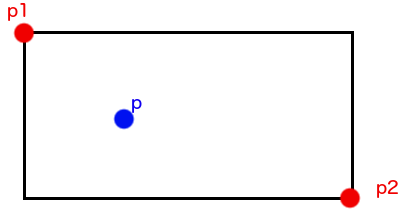
\includegraphics[width=0.7\linewidth]{box}
	\end{figure}
	\begin{lstlisting}
boolean inBox(Point p1, Point p2, Point p) {
    return 
        Math.min(p1.x, p2.x) <= p.x && 
        p.x <= Math.max(p1.x, p2.x) &&			           
        Math.min(p1.y, p2.y) <= p.y && 
        p.y <= Math.max(p1.y, p2.y);
}
	\end{lstlisting}
\end{frame}

\begin{frame}
	\frametitle{Lines}
	General formula:
	$$Ax+By=C$$
	
	The line through $(x_1,y_1),(x_2,y_2)$ is given by:
	$$A=y_2-y_1$$
	$$B=x_1-x_2$$
	$$C=Ax_1+Bx_2$$
\end{frame}

\begin{frame}
	\frametitle{Distance from a point to a line}
	Euclidian distance from a point $(x_0,y_0)$ to a line $Ax+By=C$ is
	$$\frac{|Ax_0+By_0+C|}{\sqrt{A^2+B^2}}$$
\end{frame}
\begin{frame}
	\frametitle{Line intersections}
	Two lines $A_1x+B_1y=C_1$ and $A_2x+B_2y=C_2$ intersects iff
	$$d := \det \begin{pmatrix}
	A_1 & B_1 \\
	A_2 & B_2 \\
	\end{pmatrix} \neq 0$$
	\pause remeber that:$$ \det \begin{pmatrix}
	A_1 & B_1 \\
	A_2 & B_2 \\
	\end{pmatrix} = A_1B_2 - A_2B_1 = d$$
	\pause
	The intersection is then given by:
	$$\begin{pmatrix}
	x\\
	y
	\end{pmatrix} = 
	\begin{pmatrix}
	A_1 & B_1 \\
	A_2 & B_2 \\
	\end{pmatrix}^{-1} 
	\begin{pmatrix}
	C_1 \\
	C_2
	\end{pmatrix}
	=
	\frac{1}{d}
	\begin{pmatrix}
	B_2 & -B_1 \\
	-A_2 & A_1 \\
	\end{pmatrix} 
	\begin{pmatrix}
	C_1 \\
	C_2
	\end{pmatrix}
	$$
\end{frame}

\begin{frame}
	\frametitle{For those who don't like matrices}
	$$\begin{pmatrix}
	x\\
	y
	\end{pmatrix} = 
	\begin{pmatrix}
	A_1 & B_1 \\
	A_2 & B_2 \\
	\end{pmatrix}^{-1} 
	\begin{pmatrix}
	C_1 \\
	C_2
	\end{pmatrix}
	=
	\frac{1}{d}
	\begin{pmatrix}
	B_2 & -B_1 \\
	-A_2 & A_1 \\
	\end{pmatrix} 
	\begin{pmatrix}
	C_1 \\
	C_2
	\end{pmatrix}
	$$
	$$\rightarrow$$
	$$x = \frac{B_2C_1-B_1C_2}{d},$$
	$$y = \frac{A_1C_2-A_2C_1}{d}$$
\end{frame}

\begin{frame}
	\frametitle{Perpendicular line in 2D}
	The line perpendicular to $Ax+By=C$ are
	$$-Bx+Ay=D \text{ for } D \in \mathbb{R}$$
	
	If you want that the line goes through $(x_0, y_0)$:
	$$D=-Bx_0+Ay_0$$
\end{frame}

\begin{frame}
	\frametitle{Orthogonal symmetry}
	For a line $a$, and a point $x$, find its orthogonal symmetry point $x'$:
	
	\begin{enumerate}
		\item Compute the perpendicular $b$ of $a$ that goes throught $x$
		\item find the intersection $y$ of $a$ and $b$
		\item $x'=y-(x-y)$
	\end{enumerate}
\end{frame}
\begin{frame}[fragile]
	\frametitle{Orientation}
	$$
	orient(p, q, r) = 
	\begin{vmatrix}
	1 & p_x & p_y \\
	1 & q_x & q_y \\
	1 & r_x & r_y
	\end{vmatrix}
	$$
	
	$$
	orient(p, q, r) \left\{
	\begin{array}{l l l}
	= 0 \quad & \text{$p, q, r$ are collinear} \\
	< 0 \quad & \text{$p$ -> $q$ -> $r$ is clockwise} \\
	> 0 \quad & \text{$p$ -> $q$ -> $r$ is counterclockwise}
	\end{array} \right.
	$$
	
	$$
	|orient(p, q, r)| = 2 \cdot area \ \triangle(p, q, r)
	$$
	
	\begin{lstlisting}
double orient(Point p, Point q, Point r) {
    return q.x * r.y - r.x * q.y - p.x * (r.y - q.y) + p.y * (r.x - q.x);
}
	\end{lstlisting}
\end{frame}

\begin{frame}
	\frametitle{Angle visibility}
	$x$ lies strictly inside the angle formed by $p, q, r$ iff
	\begin{align*}
	sgn(orient(p, q, x)) & = sgn(orient(p, x, r)) \\
	sgn(orient(p, r, x)) & = sgn(orient(p, x, q)) \\
	\end{align*}
	To allow it to lie on the border simply check if $$sgn(orient(p, q, x)) = 0 \text{ or } sgn(orient(p, r, x)) = 0$$
\end{frame}

\begin{frame}
	\frametitle{Triangles}
	Notations and definitions:
	\begin{itemize}
		\item sides a, b, c
		\item angles $\alpha$, $\beta$, $\gamma$
		\item perimeter $p = a+b+c$
		\item semi-perimeter $s=\frac{p}{2}$
		\item Area $$A=\frac{\text{base}*\text{height}}{2}$$
		\item Heron's formula
		$$A=\sqrt{s(s-a)(s-b)(s-c)}$$
	\end{itemize}
\end{frame}

\begin{frame}
	\frametitle{Triangles (2)}
	\begin{itemize}
		\item Inscribed circle radius
			$$r=\frac{A}{s}$$
		\item Center of inscribed circle: intersection of the bisectors of the angles
		\item Circumscribed circle radius:
			$$R=\frac{abc}{4A}$$
		\item Center of circumscribed circle:
			intersection of the perpendicular bisectors
	\end{itemize}
\end{frame}

\begin{frame}
	\frametitle{Triangles (3)}
	\begin{itemize}
		\item Law of sines
			$$\frac{a}{\sin(\alpha)} = \frac{b}{\sin(\beta)} = \frac{c}{\sin(\gamma)}=2R$$
		\item Law of cosines
			$$c^2=a^2+b^2-2ab\cos(\gamma)$$
	\end{itemize}
\end{frame}

\begin{frame}
	\frametitle{Circles}
	Definitions and notations
	\begin{itemize}
		\item Radius $r$ and center $c = (a,b)$
		\item Equation that point on the circle respects: 
		$$(x-a)^2+(y-b)^2=r^2$$
		\item Diameter $$D=2r$$
		\item Area $$A= \pi r^2$$
		\item Perimeter $$p = 2\pi r$$ (also called circumference)
		
	\end{itemize}
\end{frame}

\begin{frame}
	\frametitle{Circles (2)}
	\begin{itemize}
		\item Arc: connected section of the circumference of the circle. Given the angle $\alpha$ made, the size of an arc is
			$$\frac{p}{\alpha}{2\pi}$$
		\item Chord: ligne segment whose endpoints are on a circle. Given the angle $\alpha$ made, the size of the chord is:
		$$\sqrt{2r^2(1-\cos(\alpha))}$$
		\item Sector: area between two radiuses and the arc between these two radiuses. Given the angle $\alpha$ made:
			$$A\frac{\alpha}{2\pi}$$
		\item Segment: sector minus the triangle made by the chord
	\end{itemize}
\end{frame}

\section{Computationnal geometry}
\begin{frame}
	\frametitle{Computationnal geometry, in one slide}
	Four things to remember
	\begin{itemize}
		\pause \item floating point operations make computation errors
		\pause \item computing on floating point lead to precision errors
		\pause \item computations on floats and doubles are nearly always approximative
		\pause \item I think you have understood
	\end{itemize}
\end{frame}

\begin{frame}[fragile]
	\frametitle{Example of error}
	\begin{lstlisting}
	printf (" %.20f \n", 3.6);
	\end{lstlisting}
	Output:
	\begin{lstlisting}
	3.60000000000000008882 
	\end{lstlisting}
\end{frame}

\begin{frame}[fragile]
	\frametitle{Handling errors}
	Define an "error threshold" $\epsilon$:
	\begin{lstlisting}
boolean eq(double a,double b){return Math.abs(a - b) <= E;}
boolean le(double a,double b){return a < b - E;}
boolean leq(double a,double b){return a <= b + E;}
	\end{lstlisting}
\end{frame}

\section{Polygons}
\begin{frame}[fragile]
	\frametitle{Storing a polygon}
	Polygon = serie of points. Store them in an ordered way, for example, clockwise.
	
	\begin{lstlisting}
	Point[] polygon;
	\end{lstlisting}
\end{frame}

\begin{frame}[fragile]
	\frametitle{Perimeter of a polygon}
	Simply iterate on all the points
	\begin{lstlisting}
	double p = 0;
	for(int i = 0; i < polygon.length; i++) {
		p += dist(polygon[i], polygon[(i+1)%polygon.length]);
	}
	\end{lstlisting}
\end{frame}

\begin{frame}
	\frametitle{Area of a polygon}
	\pause Idea: get the area below all successive pair of points, and add/substract it depending on orientation
\end{frame}

\begin{frame}
	\frametitle{Area of a polygon (2)}
	\begin{figure}
		\centering
		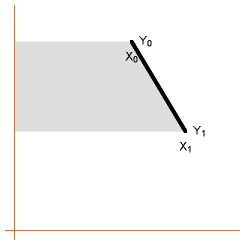
\includegraphics[width=0.7\linewidth]{area1}
	\end{figure}
\end{frame}

\begin{frame}
	\frametitle{Area of a polygon (3)}
	\begin{figure}
		\centering
		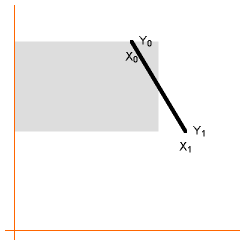
\includegraphics[width=0.7\linewidth]{area2}
	\end{figure}
\end{frame}

\begin{frame}
	\frametitle{Area of a polygon (4)}
	\begin{figure}
		\centering
		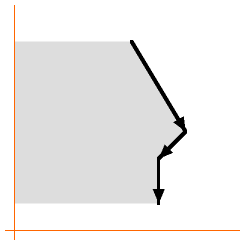
\includegraphics[width=0.7\linewidth]{area3}
	\end{figure}
\end{frame}

\begin{frame}
	\frametitle{Area of a polygon (5)}
	\begin{figure}
		\centering
		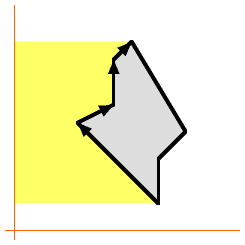
\includegraphics[width=0.7\linewidth]{area4}
	\end{figure}
\end{frame}


\begin{frame}
	\frametitle{Area of a polygon (6)}
	$$A=\frac{1}{2}\begin{vmatrix}
	x_0 & y_0 \\
	x_1 & y_1 \\
	x_2 & y_2 \\
	... & ... \\
	x_n & y_n \\
	\end{vmatrix}=\frac{1}{2}*(x_0y_1+x_1y_2+...+x_ny_0-x_1y_0-x_2y_1-...-x_0y_n)$$
\end{frame}

\begin{frame}[fragile]
	\frametitle{Area of a polygon (7)}
	\begin{lstlisting}
	double result = 0;
	for(int i = 0; i < polygon.length()-1; i++) {
		result += (P[i].x * P[i+1].y - P[i+1].x * P[i].y);
	}
	\end{lstlisting}
\end{frame}

\begin{frame}
	\frametitle{Checking if a polygon is convex}
	$\rightarrow$ check that \textit{orient(p,q,r)} is always positive for all successive triplet of points
\end{frame}

\begin{frame}
	\frametitle{Check if point is inside a polygon}
	$\rightarrow$ compute the angle made by all the successive pairs of points and the point we want to check. If it is 360 degrees, the point is inside the polygon.
	
	\begin{figure}
		\centering
		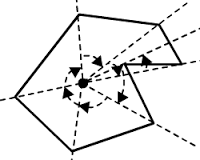
\includegraphics[width=0.7\linewidth]{winding}
	\end{figure}
\end{frame}

\section{Convex hull}
\begin{frame}
	\frametitle{Convex Hull}
	Given a set of points in the plane, compute the smallest convex polygon in the plane that contains all the points.
\end{frame}

\begin{frame}
	\frametitle{Graham Scan}
	Method of computing the convex hull of a finite set of points in the plane with time complexity O(n log(n)). The algorithm finds all vertices of the convex hull ordered along its boundary.
\end{frame}

\begin{frame}
	\frametitle{Graham Scan}
	\framesubtitle{Idea}
	\begin{itemize}
		\item find the point with the lowest y-coordinate. if there are multiple points with the lowest y-coordinate, the pick that one of them with the lowest x-coordinate. call this point P
		\item now sort all the points in increasing order of the angle they and point P make with the x-axis
		\item consider each point in the sorted array in sequence. For each point determine whether coming from the 2 previous points it makes a left of a right turn.
		\item if it makes a left turn, proceed with the next point
		\item if it makes a right turn, the second-to-last point is not part of the convex hull and should be removed from the convex hull, continue this removing for as long as the last 3 points make up a right turn 
	\end{itemize}
\end{frame}

\begin{frame}
	\frametitle{Graham Scan}
	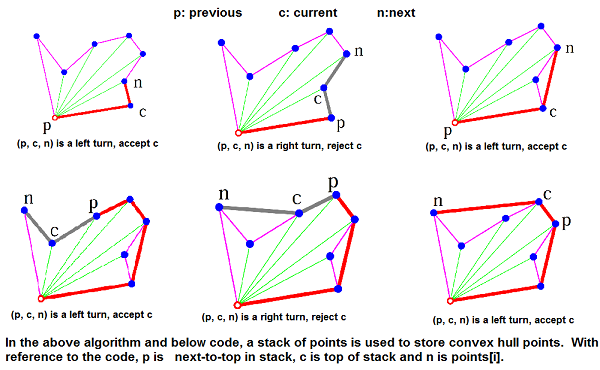
\includegraphics[width=1\textwidth]{graham}
\end{frame}

\begin{frame}
	\frametitle{Graham Scan}
	\framesubtitle{Direction of the turn}
	To determine whether 3 points constitute a left or a right turn we do not have to compute the actual angles but we can use a cross product.\\
	Consider the 3 points $(x_{1}, y_{1})$,  $(x_{2}, y_{2})$ and $(x_{3}, y_{3})$, which we will call $P_{1}, P_{2}$ and $P_{3}$.\\
	Now compute the z-component of the cross product of the vectors $P_{1}P_{2}$ and $P_{1}P_{3}$. Which is given by the expression $(x_{2}-x_{1})(y_{3}-y_{1})-(y_{2}-y_{1})(x_{3}-x_{1})$.\\
	If the result is 0, the points are collinear. If the result is positive, the 3 points constitute a left turn. If the result is negative, the 3 points constitute a right turn.
\end{frame}

\begin{frame}[fragile]
	\frametitle{Sorting points by angle}
	Here is a comparator (in C++)
	\begin{lstlisting}
		point pivot(0, 0);
		bool angleCmp(point a, point b) {
			if(orient(pivot, a, b) == 0) //collinear: return the closer one
				return dist(pivot, a) < dist(pivot, b);
			double d1x = a.x - pivot.x, d1y = a.y - pivot.y;
			double d2x = b.x - pivot.x, d2y = b.y - pivot.y;
			return (atan2(d1y, d1x) - atan2(d2y, d2x)) < 0; //compare angles
		}
	\end{lstlisting}
\end{frame}

\begin{frame}
	\frametitle{Exercices}
	Do them in this order!
	\begin{itemize}
		\item 634
		\item 10060
		\item 478
		\item 681
		\item 109
	\end{itemize}
\end{frame}
\end{document}